% vim: set spell spelllang=es syntax=tex :

\section{Metodología experimental}

Para comprobar el funcionamiento del nuevo framework se grabo un vídeo a partir
del cual se crearon dos, uno con una resolución de 800x600 píxeles y otro con
una resolución de 1280x720 píxeles.

Se configuraron diferentes experimentos haciendo variar la cantidad de partes en
las que fueron divididos los cuadros entre 1 y 24, la cantidad de hilos de
ejecución para tareas dinámicas entre 1 y 12, con ambos vídeos. Para comparar
los resultados de las diferentes configuraciones se midieron los \emph{FPS}
soportados por el sistema y el tiempo de espera máximo (obtenido a los
\emph{FPS} soportados por el sistema bajo la misma configuración).

Como la obtención del retardo máximo depende del conocimiento previo de los
\emph{FPS}, cada experimento se dividió en dos partes. En la primera parte se
busca la cantidad de \emph{FPS} soportados por el sistema para esa
configuración. Para esto, el programa procesa tantos cuadros del vídeo como
pueda en un cierto intervalo de tiempo. En la segunda parte se limita la
cantidad de cuadros por segundo (según el valor de \emph{FPS} encontrado en la
primera parte del experimento) y se registra el tiempo de espera máximo. Dado
que se trata de un sistema de tiempo real, es importante determinar las cotas
inferiores del rendimiento. Por esto, se repitió cada experimento 10 veces,
registrando sólo el peor valor obtenido para cada variable en cada
configuración.

Dada la gran cantidad de ejecuciones se busco el tiempo mínimo necesario para
que estas fueran representativas de una ejecución prolongada. Se realizaron 3
ejecuciones con 11 hilos y 10 fragmento procesando el vídeo 800x600 píxeles de
resolución, durante 6 minutos. El primer minuto no se contabilizo con el fin de
permitir que la ejecución se estabilizara. Estas se compararon con ejecuciones
bajo la misma configuración, pero ejecutando de 11 a 20 segundos, y
contabilizando solo los últimos 10. Para poder realizar la prueba de 6 minutos
se tuvo que modificar el sistema para que reutilizaran los cuadros, es por esto
que los resultados de esta prueba no coinciden con los de las pruebas finales.
Con esta prueba se pudo comprobar que las pruebas de 16 segundos son
representativas de ejecuciones mas largas. En la siguiente tabla se pueden ver
los resultados de estas pruebas.

Dada la gran cantidad de experimentos, se buscó el tiempo mínimo de ejecución
necesario para que éstos fueran representativos de una ejecución prolongada. Se
realizaron tres ejecuciones de 6 minutos cada una con una misma configuración:
11 hilos y 10 fragmentos procesando el vídeo de 800x600 píxeles de resolución.
El primer minuto no se contabilizó, con el fin de permitir que la ejecución se
estabilizara. Los resultados se compararon con ejecuciones bajo la misma
configuración, pero ejecutando de 11 a 20 segundos, y contabilizando sólo los
últimos 10 segundos. En la tabla 1 se muestran los \emph{FPS} obtenidos para
cada ejecución. Se observa que las pruebas de 16 segundos son representativas de
ejecuciones más largas. Dado que los 6 minutos de vídeo no caben en la memoria
RAM del equipo de pruebas, el sistema fue modificado para reintroducir en la
lista de cuadros a procesar aquellos cuadros ya procesados. Debido a esto, el
rendimiento en estos experimentos es levemente inferior al resto con igual
configuración.

\begin{table}[h]
	\centering
	\begin{tabular}{c|c|c|c|c|c|c|c|c|c|c|c}

		Ejecución&6min&11s&12s&13s&14s&15s&16s&17s&18s&19s&20s\\

		\hline

		1&166& 171& 170& 170& 170& 169& 166& 166& 166& 166& 165\\

		\hline

		2&166& 171& 170& 170& 170& 168& 167& 166& 166& 165& 166\\

		\hline

		3&166& 171& 170& 170& 170& 169& 166& 166& 167& 166& 165

	\end{tabular}

	\caption{Búsqueda de la duración mínima de los experimentos}

\label{tabla}

\end{table}

\section{Plataforma experimental}

El equipo de pruebas cuenta un procesador Intel Xeon E5-2630. Este es un
procesador de 6 núcleos con multithreading simultáneo de dos vías, una
frecuencia básica de CPU de 2,30GHz y 2,8GHz en modo turbo, 15MiB de memoria
caché L3, 256KiB de caché L2, 32Kib de caché L1 para datos, y 32 KiB de caché L1
para instrucciones. El equipo posee ademas con 16GiB de memoria RAM. La
jerarquía de memoria se muestra en la figura \ref{topoMemoria}

\begin{figure}[!ht]

	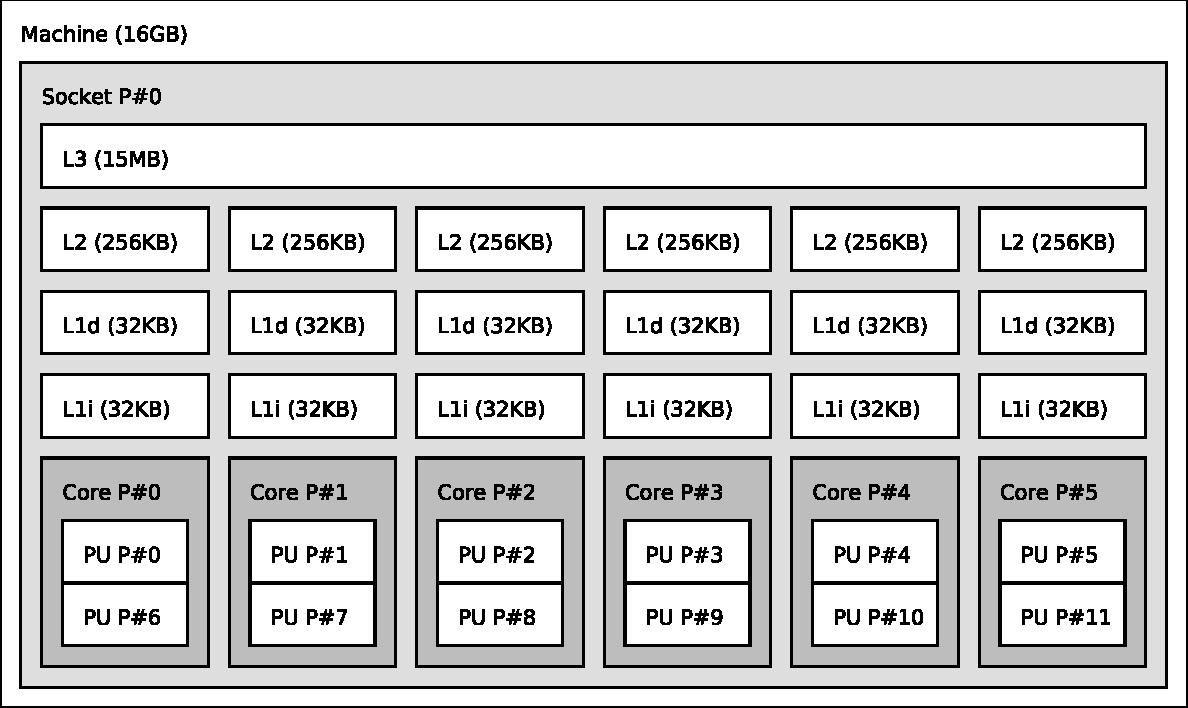
\includegraphics[width=\textwidth]{img/topo.pdf}
	\caption{Jerarquía de memoria de la maquina de pruebas.}

	\label{topoMemoria}

\end{figure}

\section{Resultados}

Durante el desarrollo de la aplicación se probaron tres distintas
implementaciones. En la primera implementación, el framework ejecutaba las
distintas pilas de plugins en tareas separadas. En la segunda implementación el
framework fue modificado para que una sola tarea ejecutara todas las pilas de
plugins sobre un mismo fragmento. Para la tercera implementación se trabajo
sobre el mismo framework que la segunda, pero se unieron las pilas de búsquedas
de robots y la de búsqueda de pelota. Para comprobar cual de estas era la mas
efectiva se realizaron las pruebas con cada una de estas para la configuración
de 11 hilos de búsqueda y 10 particiones con el vídeo de 800x600 píxeles de
resolución. La primera implementación proceso XX \emph{FPS}, la segunda XX
\emph{FPS} y la tercera 188 \emph{FPS}. Como esta última fue la que produjo
resultados mas satisfactorios, sera sobre los resultados de esta que
trabajaremos a continuación.

NOTA: Faltan los datos, los consigo mañana.

En las figuras \ref{800fps} y \ref{1280fps} se muestran las cantidades de
\emph{FPS} alcanzados para un vídeo de 800x600 píxeles y 1280x720 píxeles
respectivamente, para distintas cantidades de hilos de búsqueda y fragmentos.
El numero de hilos de búsqueda indica la cantidad de hilos que ejecutan las
tareas dinámicas. Adicionalmente el sistema ejecuta dos hilos más para las
tareas estáticas, uno para la generación de cuadros y otro para la tarea de
generación de tareas dinámicas. En el caso de del vídeo de 800x600 píxeles se
llego a un máximo de 195 \emph{FPS} cuando se divide el cuadro en 18 fragmentos
y se utilizan 10 u 11 hilos de búsqueda, mientras que para el vídeo de 1280x720
píxeles se alcanzo un máximo de 94 \emph{FPS} cuando se divide el cuadro en 21
fragmentos y se utilizan 10 u 11 cuadros de búsqueda.

\begin{figure}[!h]

	\includegraphics[width=\textwidth]{img/800x600_fps.pdf}
	\caption{FPS alcanzados por el sistema para vídeo de 800x600 píxeles}
	\label{800fps}

\end{figure}

\begin{figure}[!h]

	\includegraphics[width=\textwidth]{img/1280x720_fps.pdf}
	\caption{FPS alcanzados por el sistema para vídeo de 1280x720 píxeles}
	\label{1280fps}

\end{figure}

En las figuras \ref{800fps} y \ref{1280fps} se pueden observar dos patrones que
ocurren en ambos vídeos. El primero es que si los cuadros se dividen en 7, 11,
17, 19 y 23 fragmentos, se produce una notable reducción en la cantidad de
cuadros por segundo con respecto a las divisiones adyacentes.

Cuando se incrementan la cantidad de fragmentos aumenta el área compartida y por
lo tanto el área total que se procesa, al mismo, una mayor cantidad de
fragmentos permite aprovechar mejor el paralelismo. Si se divide el cuadro en un
número primo de fragmentos, el área total se incrementa de forma significativa
con respecto a los valores circundantes. En la figura \ref{primosArea} se
muestra la fluctuación del área para cada cantidad de particiones desde 1 hasta
100 para un vídeo de 1280x720 píxeles de resolución, resaltando el crecimiento
para valores primos y para los valores inmediatamente inferiores y superiores.
Como puede observarse, a partir de 7 fragmentos el área total se incrementa de
forma significativa cuando el número es primo con respecto a los valores
cercanos no primos. Esto lleva a que un cambio mínimo en las posibilidades de
aprovechar el paralelismo se vea acompañado por un gran incremento en el área a
procesar.

Esto se produce porque cuando los cuadros se dividen en un número primo de
fragmentos, el área total a procesar se incrementa de forma significativa con
respecto a los valores circundantes. En la figura \ref{primosArea} se muestra la
fluctuación de la suma del área de los fragmentos en divisiones de 1 hasta 100
fragmentos para un vídeo de 1280x720 píxeles de resolución, resaltando los
resultados para valores primos y para los valores inmediatamente inferiores y
superiores. Como puede observarse, a partir de 7 fragmentos el área total se
incrementa de forma significativa cuando el número es primo con respecto a los
valores cercanos con divisores. En estos casos, un incremento del número
de fragmentos aumenta el paralelismo, pero es acompañado de un incremento
drástico del área a procesar.

\begin{figure}[!h]

	\includegraphics[width=\textwidth]{img/primos_area.pdf}
	\caption{Área total a procesar para número de fragmentos primos y sus inmediatos}
	\label{primosArea}

\end{figure}

Para comprobar como esta variación de volumen de datos afecta la cantidad de
cuadros por segundo procesados, se realizaron nuevas pruebas sobre el vídeo de
1280x720 píxeles de resolución, con 11 hilos de búsqueda y variando la cantidad
de fragmentos entre los números primos mayores a 24 y menores a 100, y sus
inmediatos superior e inferior. Los valores para números primos e inmediatos
inferiores a 24 fueron tomados de los experimentos anteriores. Los resultados
pueden ser observados en la figura \ref{primosFPS}.

\begin{figure}[!h]

	\includegraphics[width=\textwidth]{img/primos_fps.pdf}
	\caption{FPS totales para número de fragmentos primos y sus inmediatos}
	\label{primosFPS}

\end{figure}

Como se puede observar en la figura, para una cantidad de fragmentos menor a 7,
el perjuicio por aumento en el área es menor que el beneficio aportado por el
incremento en el paralelismo. Si se observa la figura \ref{primosArea}, dividir
el cuadro en 7 fragmentos resulta en el primer incremento notable de área con
respecto tanto a un fragmento menos como un fragmento más. También se pueden
apreciar que los incrementos repentinos en el área total coinciden con
disminuciones repentinas en los cuadros por segundo procesados.

El segundo patrón
que se puede observar es una reducción en la cantidad de cuadros por segundo
cuando la cantidad de fragmentos es reducida y la cantidad de hilos de búsqueda
alta.

El segundo patrón que se puede observar en las figuras \ref{800fps} y
\ref{1280fps} es que cuando la cantidad de fragmentos es baja y la cantidad de
hilos de búsqueda es alta, el sistema tiene menor \emph{FPS} que utilizar una
menor cantidad de hilos búsqueda pero una mayor cantidad de fragmentos. La
memoria caché se comparte entre los cuadros que están siendo procesados en
paralelo. Cuanto más cuadros se procesen en paralelo, mayor será la competencia
por la memoria caché. La cantidad de cuadros que se procesan en paralelo está en
relación con el número de fragmentos y la cantidad de hilos de ejecución para
tareas dinámicas. Considerando que la cantidad de hilos de ejecución es mayor
que la cantidad de fragmentos, si se disminuye la cantidad de fragmentos,
manteniendo la cantidad de hilos de ejecución para tareas dinámicas, se
incrementa la cantidad de cuadros a procesar en paralelo. Esto tiene como
efecto que los cuadros compitan por la caché y reduce las posibilidades de que
los fragmentos entren completamente en las cachés de nivel mas bajo. Por esto se
propuso la hipótesis de que el retardo se produce debido a un aumento en los
fallos de caché.

Para comprobar que la hipótesis es correcta se diseñó el siguiente experimento.
Se ejecutó el programa procesando cuadros de un vídeo de 1280x720 píxeles de
resolución, y se midieron los fallos de caché en configuraciones de 1, 2, 6 y 12
fragmentos y cantidad de hilos búsqueda de 1 a 11. Para obtener los fallos de
caché de nivel 3 (es decir, cuando es necesario acceder a datos en la memoria
RAM) se utilizó la herramienta \emph{perf}. Ésta es una aplicación que permite
acceder a los contadores de hardware del procesador que proveen datos muy
precisos con un overhead despreciable.

En la figura \ref{cacheFallos} se muestran los fallos de caché por cuadro
obtenidos en el experimento. Como se puede apreciar, a menor cantidad de
fragmentos, mayor es la cantidad de fallos de caché ocurridos por cuadro.

\begin{figure}[!h]

	\includegraphics[width=\textwidth]{img/cache_fallos.pdf}
	\caption{Fallos de caché por cuadro para distintas cantidades de
	fragmentos}
	\label{cacheFallos}

\end{figure}

Finalmente, en las figuras \ref{800turnArround} y \ref{1280turnArround} se
muestran los tiempos máximos de espera de los cuadros, para los vídeos de
800x600 y 1280x720 píxeles de resolución (considerando que los \emph{FPS} son
limitados al máximo encontrado en la primera etapa de los experimentos).

\begin{figure}[!h]

	\includegraphics[width=\textwidth]{img/800x600_turnArround.pdf}
	\caption{Tiempos máximos de espera para vídeo de 800x600 píxeles}
	\label{800turnArround}

\end{figure}


\begin{figure}[!h]

	\includegraphics[width=\textwidth]{img/1280x720_turnArround.pdf}
	\caption{Tiempos máximos de espera para vídeo de 1280x720 píxeles}
	\label{1280turnArround}

\end{figure}

Estos dos últimas figuras nos permiten apreciar que no siempre una mayor
cantidad de cuadros por segundos procesados implicara el tiempo de espera
mínimo. Dependiendo de si se desea minimizar el tiempo de espera de los cuadros,
maximizar la cantidad de cuadros procesados, o encontrar un balance especifico,
se deberá elegir una cantidad de fragmentos y procesadores apropiada. Por
ejemplo, en el caso del vídeo de 1280x720 píxeles de resolución, dividir la
imagen en 21 fragmentos y utilizar 11 permite procesar 94 cuadros por segundo en
el equipo de prueba, sin embargo el tiempo de espera es de $0.09$ segundos. Si
el cuadro se divide en 15 fragmentos y se utilizan 11 hilos de búsqueda, la
cantidad de cuadros por segundo procesados se cae a 90, pero el tiempo de espera
se reduce a $0.05$ segundos. Las figuras \ref{800tFPS} y \ref{1280tFPS}
sintetizan la relación entre los \emph{FPS} y el retardo de cuadros, mostrando
el mínimo retardo de cuadros para los diferentes \emph{FPS} que puede alcanzar
el sistema en cada vídeo.

\begin{figure}[!h]

	\includegraphics[width=\textwidth]{img/800x600_tFPS.pdf}
	\caption{Tiempos máximos de espera para vídeo de 800x600 píxeles para
	los FPS soportados por el sistema}
	\label{800tFPS}

\end{figure}

\begin{figure}[!h]

	\includegraphics[width=\textwidth]{img/1280x720_tFPS.pdf}
	\caption{Tiempos máximos de espera para vídeo de 1280x720 píxeles para
	los FPS soportados por el sistema}
	\label{1280tFPS}

\end{figure}
